\documentclass{standalone}
\usepackage{tikz}
\usetikzlibrary{patterns, positioning}

\begin{document}
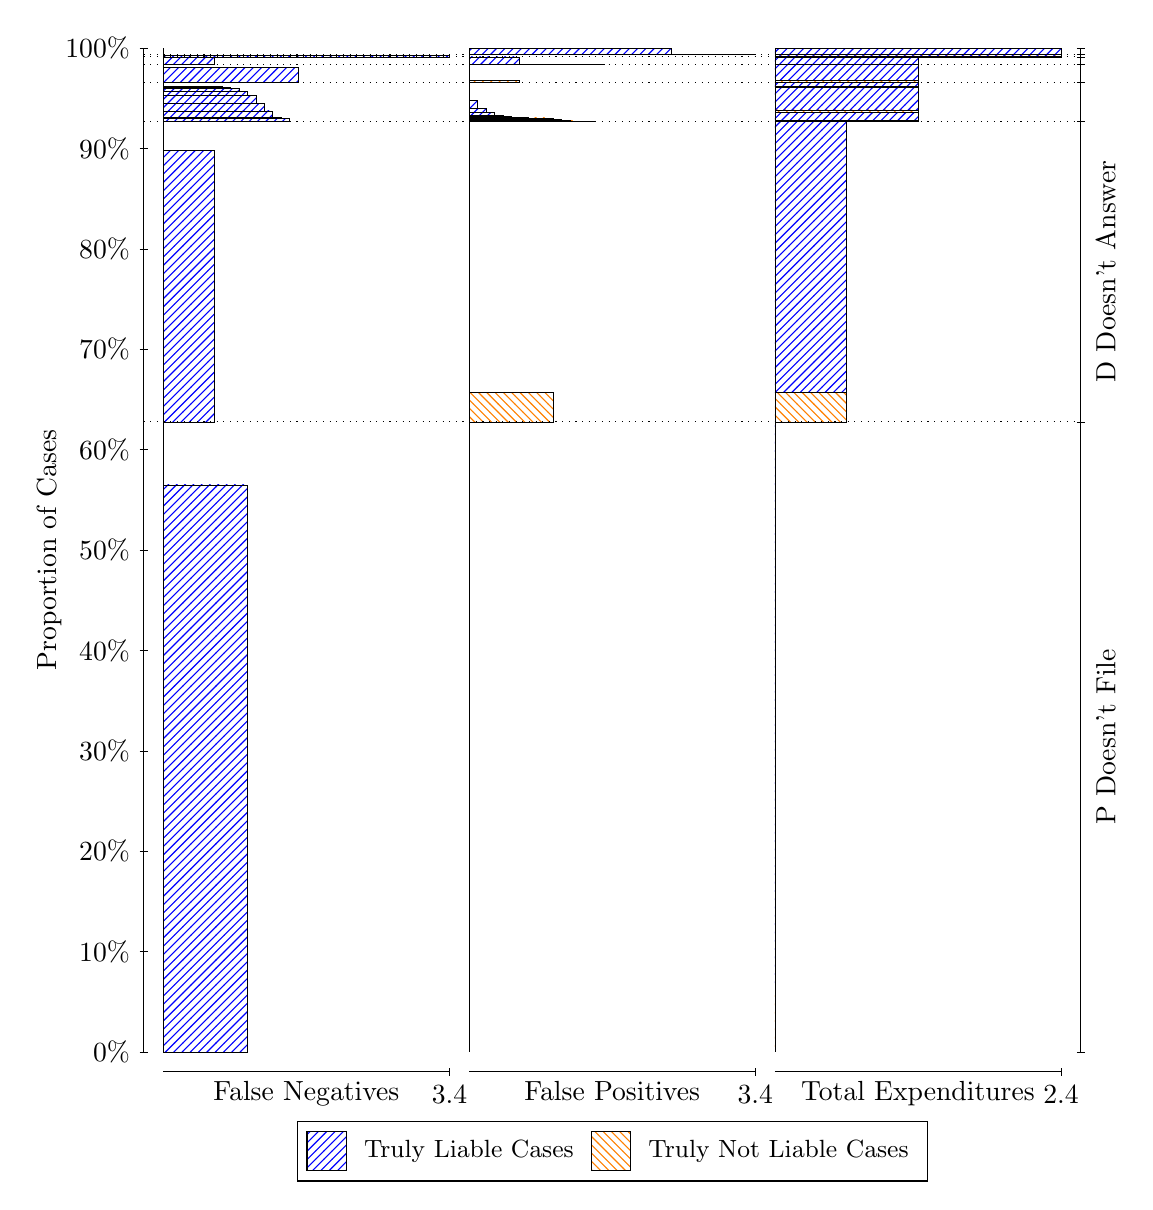
\begin{tikzpicture}
\draw[black, very thin] (1.5,1.75) -- (1.5,14.5);
\node[rotate=90, anchor=center] at (0.3, 8.125) {Proportion of Cases};
\draw[black, very thin] (1.45,1.75) -- (1.55,1.75);
\node[anchor=east] at (1.45, 1.75) {0\%};
\draw[black, very thin] (1.45,3.025) -- (1.55,3.025);
\node[anchor=east] at (1.45, 3.025) {10\%};
\draw[black, very thin] (1.45,4.3) -- (1.55,4.3);
\node[anchor=east] at (1.45, 4.3) {20\%};
\draw[black, very thin] (1.45,5.575) -- (1.55,5.575);
\node[anchor=east] at (1.45, 5.575) {30\%};
\draw[black, very thin] (1.45,6.85) -- (1.55,6.85);
\node[anchor=east] at (1.45, 6.85) {40\%};
\draw[black, very thin] (1.45,8.125) -- (1.55,8.125);
\node[anchor=east] at (1.45, 8.125) {50\%};
\draw[black, very thin] (1.45,9.4) -- (1.55,9.4);
\node[anchor=east] at (1.45, 9.4) {60\%};
\draw[black, very thin] (1.45,10.675) -- (1.55,10.675);
\node[anchor=east] at (1.45, 10.675) {70\%};
\draw[black, very thin] (1.45,11.95) -- (1.55,11.95);
\node[anchor=east] at (1.45, 11.95) {80\%};
\draw[black, very thin] (1.45,13.225) -- (1.55,13.225);
\node[anchor=east] at (1.45, 13.225) {90\%};
\draw[black, very thin] (1.45,14.5) -- (1.55,14.5);
\node[anchor=east] at (1.45, 14.5) {100\%};

\draw[black, very thin] (13.4,1.75) -- (13.4,14.5);
\draw[black, very thin] (13.35,1.75) -- (13.45,1.75);
\node[anchor=west] at (13.35, 1.75) {};
\draw[black, very thin] (13.35,9.7528) -- (13.45,9.7528);
\node[anchor=west] at (13.35, 9.7528) {};
\draw[black, very thin] (13.35,13.569) -- (13.45,13.569);
\node[anchor=west] at (13.35, 13.569) {};
\draw[black, very thin] (13.35,14.059) -- (13.45,14.059);
\node[anchor=west] at (13.35, 14.059) {};
\draw[black, very thin] (13.35,14.289) -- (13.45,14.289);
\node[anchor=west] at (13.35, 14.289) {};
\draw[black, very thin] (13.35,14.388) -- (13.45,14.388);
\node[anchor=west] at (13.35, 14.388) {};
\draw[black, very thin] (13.35,14.422) -- (13.45,14.422);
\node[anchor=west] at (13.35, 14.422) {};
\draw[black, very thin] (13.35,14.5) -- (13.45,14.5);
\node[anchor=west] at (13.35, 14.5) {};

\draw[black, very thin, pattern color=blue, pattern=north east lines] (1.75,1.75) rectangle (2.8186,8.9525);
\draw[black, very thin, pattern color=orange, pattern=north west lines] (1.75,8.9525) rectangle (1.75,9.7528);
\draw[black, very thin, pattern color=blue, pattern=north east lines] (1.75,9.7528) rectangle (2.3912,13.199);
\draw[black, very thin, pattern color=orange, pattern=north west lines] (1.75,13.199) rectangle (1.75,13.569);
\draw[black, very thin, pattern color=blue, pattern=north east lines] (1.75,13.569) rectangle (3.3529,13.605);
\draw[black, very thin, pattern color=blue, pattern=north east lines] (1.75,13.605) rectangle (3.2461,13.624);
\draw[black, very thin, pattern color=blue, pattern=north east lines] (1.75,13.624) rectangle (3.1392,13.703);
\draw[black, very thin, pattern color=blue, pattern=north east lines] (1.75,13.703) rectangle (3.0324,13.797);
\draw[black, very thin, pattern color=blue, pattern=north east lines] (1.75,13.797) rectangle (2.9255,13.896);
\draw[black, very thin, pattern color=blue, pattern=north east lines] (1.75,13.896) rectangle (2.8186,13.949);
\draw[black, very thin, pattern color=blue, pattern=north east lines] (1.75,13.949) rectangle (2.7118,13.983);
\draw[black, very thin, pattern color=blue, pattern=north east lines] (1.75,13.983) rectangle (2.6049,13.996);
\draw[black, very thin, pattern color=blue, pattern=north east lines] (1.75,13.996) rectangle (2.498,14.009);
\draw[black, very thin, pattern color=orange, pattern=north west lines] (1.75,14.009) rectangle (1.75,14.059);
\draw[black, very thin, pattern color=blue, pattern=north east lines] (1.75,14.059) rectangle (3.4598,14.258);
\draw[black, very thin, pattern color=orange, pattern=north west lines] (1.75,14.258) rectangle (1.75,14.289);
\draw[black, very thin, pattern color=blue, pattern=north east lines] (1.75,14.289) rectangle (2.3912,14.38);
\draw[black, very thin, pattern color=orange, pattern=north west lines] (1.75,14.38) rectangle (1.75,14.388);
\draw[black, very thin, pattern color=blue, pattern=north east lines] (1.75,14.388) rectangle (5.3833,14.409);
\draw[black, very thin, pattern color=orange, pattern=north west lines] (1.75,14.409) rectangle (1.75,14.422);
\draw[black, very thin, pattern color=orange, pattern=north west lines] (1.75,14.422) rectangle (1.75,14.424);
\draw[black, very thin, pattern color=blue, pattern=north east lines] (1.75,14.424) rectangle (1.75,14.5);
\draw[black, very thin, pattern color=orange, pattern=north west lines] (5.6333,1.75) rectangle (5.6333,2.5503);
\draw[black, very thin, pattern color=blue, pattern=north east lines] (5.6333,2.5503) rectangle (5.6333,9.7528);
\draw[black, very thin, pattern color=orange, pattern=north west lines] (5.6333,9.7528) rectangle (6.702,10.123);
\draw[black, very thin, pattern color=blue, pattern=north east lines] (5.6333,10.123) rectangle (5.6333,13.569);
\draw[black, very thin, pattern color=orange, pattern=north west lines] (5.6333,13.569) rectangle (7.2363,13.57);
\draw[black, very thin, pattern color=orange, pattern=north west lines] (5.6333,13.57) rectangle (7.1294,13.572);
\draw[black, very thin, pattern color=orange, pattern=north west lines] (5.6333,13.572) rectangle (7.0225,13.576);
\draw[black, very thin, pattern color=orange, pattern=north west lines] (5.6333,13.576) rectangle (6.9157,13.583);
\draw[black, very thin, pattern color=orange, pattern=north west lines] (5.6333,13.583) rectangle (6.8088,13.593);
\draw[black, very thin, pattern color=orange, pattern=north west lines] (5.6333,13.593) rectangle (6.702,13.602);
\draw[black, very thin, pattern color=orange, pattern=north west lines] (5.6333,13.602) rectangle (6.5951,13.612);
\draw[black, very thin, pattern color=orange, pattern=north west lines] (5.6333,13.612) rectangle (6.4882,13.614);
\draw[black, very thin, pattern color=orange, pattern=north west lines] (5.6333,13.614) rectangle (6.3814,13.62);
\draw[black, very thin, pattern color=blue, pattern=north east lines] (5.6333,13.62) rectangle (6.1676,13.632);
\draw[black, very thin, pattern color=blue, pattern=north east lines] (5.6333,13.632) rectangle (6.0608,13.645);
\draw[black, very thin, pattern color=blue, pattern=north east lines] (5.6333,13.645) rectangle (5.9539,13.679);
\draw[black, very thin, pattern color=blue, pattern=north east lines] (5.6333,13.679) rectangle (5.8471,13.732);
\draw[black, very thin, pattern color=blue, pattern=north east lines] (5.6333,13.732) rectangle (5.7402,13.831);
\draw[black, very thin, pattern color=blue, pattern=north east lines] (5.6333,13.831) rectangle (5.6333,14.059);
\draw[black, very thin, pattern color=orange, pattern=north west lines] (5.6333,14.059) rectangle (6.2745,14.09);
\draw[black, very thin, pattern color=blue, pattern=north east lines] (5.6333,14.09) rectangle (5.6333,14.289);
\draw[black, very thin, pattern color=orange, pattern=north west lines] (5.6333,14.289) rectangle (7.3431,14.297);
\draw[black, very thin, pattern color=blue, pattern=north east lines] (5.6333,14.297) rectangle (6.2745,14.388);
\draw[black, very thin, pattern color=orange, pattern=north west lines] (5.6333,14.388) rectangle (5.6333,14.4);
\draw[black, very thin, pattern color=blue, pattern=north east lines] (5.6333,14.4) rectangle (5.6333,14.422);
\draw[black, very thin, pattern color=orange, pattern=north west lines] (5.6333,14.422) rectangle (9.2667,14.424);
\draw[black, very thin, pattern color=blue, pattern=north east lines] (5.6333,14.424) rectangle (8.198,14.5);
\draw[black, very thin, pattern color=orange, pattern=north west lines] (9.5167,1.75) rectangle (9.5167,2.5503);
\draw[black, very thin, pattern color=blue, pattern=north east lines] (9.5167,2.5503) rectangle (9.5167,9.7528);
\draw[black, very thin, pattern color=orange, pattern=north west lines] (9.5167,9.7528) rectangle (10.425,10.123);
\draw[black, very thin, pattern color=blue, pattern=north east lines] (9.5167,10.123) rectangle (10.425,13.569);
\draw[black, very thin, pattern color=orange, pattern=north west lines] (9.5167,13.569) rectangle (11.333,13.579);
\draw[black, very thin, pattern color=blue, pattern=north east lines] (9.5167,13.579) rectangle (11.333,13.678);
\draw[black, very thin, pattern color=orange, pattern=north west lines] (9.5167,13.678) rectangle (11.333,13.713);
\draw[black, very thin, pattern color=blue, pattern=north east lines] (9.5167,13.713) rectangle (11.333,14.006);
\draw[black, very thin, pattern color=orange, pattern=north west lines] (9.5167,14.006) rectangle (11.333,14.012);
\draw[black, very thin, pattern color=blue, pattern=north east lines] (9.5167,14.012) rectangle (11.333,14.059);
\draw[black, very thin, pattern color=orange, pattern=north west lines] (9.5167,14.059) rectangle (11.333,14.09);
\draw[black, very thin, pattern color=blue, pattern=north east lines] (9.5167,14.09) rectangle (11.333,14.289);
\draw[black, very thin, pattern color=orange, pattern=north west lines] (9.5167,14.289) rectangle (11.333,14.297);
\draw[black, very thin, pattern color=blue, pattern=north east lines] (9.5167,14.297) rectangle (11.333,14.388);
\draw[black, very thin, pattern color=orange, pattern=north west lines] (9.5167,14.388) rectangle (13.15,14.4);
\draw[black, very thin, pattern color=blue, pattern=north east lines] (9.5167,14.4) rectangle (13.15,14.422);
\draw[black, very thin, pattern color=orange, pattern=north west lines] (9.5167,14.422) rectangle (13.15,14.424);
\draw[black, very thin, pattern color=blue, pattern=north east lines] (9.5167,14.424) rectangle (13.15,14.5);
\draw[black, dotted] (1.5,9.7528) -- (13.4,9.7528);
\draw[black, dotted] (1.5,13.569) -- (13.4,13.569);
\draw[black, dotted] (1.5,14.059) -- (13.4,14.059);
\draw[black, dotted] (1.5,14.289) -- (13.4,14.289);
\draw[black, dotted] (1.5,14.388) -- (13.4,14.388);
\draw[black, dotted] (1.5,14.422) -- (13.4,14.422);
\draw[black, very thin] (1.75,1.5) -- (5.3833,1.5);
\node[anchor=north] at (3.5667, 1.5) {False Negatives};
\draw[black, very thin] (5.3833,1.45) -- (5.3833,1.55);
\node[anchor=north] at (5.3833, 1.45) {3.4};

\draw[black, very thin] (5.6333,1.5) -- (9.2667,1.5);
\node[anchor=north] at (7.45, 1.5) {False Positives};
\draw[black, very thin] (9.2667,1.45) -- (9.2667,1.55);
\node[anchor=north] at (9.2667, 1.45) {3.4};

\draw[black, very thin] (9.5167,1.5) -- (13.15,1.5);
\node[anchor=north] at (11.333, 1.5) {Total Expenditures};
\draw[black, very thin] (13.15,1.45) -- (13.15,1.55);
\node[anchor=north] at (13.15, 1.45) {2.4};

\node[black, centered, rotate=90] at (13.72, 5.7514) {P Doesn't File};
\node[black, centered, rotate=90] at (13.72, 11.661) {D Doesn't Answer};






\draw (7.449999999999999,1.5) node[draw=none] (baseCoordinate) {};
\begin{scope}[align=center]
        \matrix[scale=0.5, draw=black, below=0.5cm of baseCoordinate, nodes={draw}, column sep=0.1cm]{
            \node[rectangle, draw, minimum width=0.5cm, minimum height=0.5cm, pattern=north east lines, pattern color=blue] {}; &
            \node[draw=none, font=\small] (B) {Truly Liable Cases}; &
            \node[rectangle, draw, minimum width=0.5cm, minimum height=0.5cm, pattern=north west lines, pattern color=orange] {}; &
            \node[draw=none, font=\small] (B) {Truly Not Liable Cases}; \\
            };
\end{scope}

\end{tikzpicture}
\end{document}